\documentclass{article}
\usepackage{geometry}[margins=1in]
\usepackage{amsmath}
\usepackage[utf8]{inputenc}
\usepackage[square, numbers, sort&compress]{natbib}
\usepackage{minted}
\usepackage{graphicx}

\bibliographystyle{abbrvnat}

\title{\texttt{bigrig}: A historical biogeography range simulator for the
	DEC[+J] model}
\author{Ben Bettisworth}

\begin{document}

\newcommand{\CountFull}[1]{|#1|_\text{full}}
\newcommand{\CountEmpty}[1]{|#1|_\text{empty}}
\newcommand{\bigrig}{\texttt{bigrig}}

\maketitle

\section{Introduction}

Verification of software for computational phylogenetics is an ever present
challenge for tool developers. 
The true phylogenetic tree, the series of speciation events starting from a
common ancestor which explains all extant species included in the phylogenetic
tree, is unobservable which renders true verification of results generated from
computational models and methods impossible.
Occasionally, researchers will obtain or create a known
phylogeny\cite{hillis_experimental_1992} which can be used to verify both models
and software for computational phylogenetics. 
However, these datasets for which the truth is known are exceptionally rare,with
only a few such datasets in existence.
Therefore, researchers cannot rely completely on these known phylogenies to
verify their tools.

However, without software verification it is difficult to tell the difference
between a surprising result, and an oversight in the software implementation
(i.e. a bug). 
Responsible tool developers must therefore turn to artificial sources of data
in order to verify the correctness of their programs.
Traditionally, artificial data is generated by assuming some statistical model
as true, and generating data based on pre-provided model parameters.
This data is unrealistic\cite{trost_simulations_2024}, as in fails to account
for the myriad complexities which present themselves when working with real
biological organisms.
Nonetheless, for the purposes of software verification, simulated artificial
data is invaluable.

The field of historical biogeography has an analogous problem.
In historical biogeography, one goal is to infer the ancestral ranges
corresponding to ancestral species.
However, these are general not observable, and certainly not in the general
case.
Therefore, a similar logic applies, and researchers must turn to simulations in
order to verify the correctness of their software.
However, simulations of biogeographical data has been done in an ad-hoc matter,
with each tool implementing their own simulation tool.
Often this is done utilizing the same computational machinery used to implement
the model.
Therefore, if there is a software error in the software, it is highly likely to
appear in the simulation as well.

Rather than implementing an ad-hoc simulation for each software project, a
better solution is to write a bespoke implementation of simulation software for
a model (or class of models).
There are several important reasons for this.
First, it is important critical that tools are assessed using a common standard.
By ensuring that a common standard is used to evaluate tools, researchers
utilizing tools can be sure that high performance isn't an artificial result of
the evaluation process.

Second, reduces repeated work for tool developers working with the particular
model.
A corollary to this is that a standard simulator lowers the amount of work
required to implement a new tool.
This has the (eventual) result of increasing the number of tools available, and
increasing the overall quality of tooling.

Third, an separation of simulation code and inference code reduces the chances
of an common error between the inference code and simulation code artificially
improving performance.

Fourth and finally, it is significantly easier to perform introspection on the
output of a well implemented simulator. 
Specifically, 


\section{Methods}

Before we describe the methods used to simulate and test the results of
\bigrig{}, we would like to define some terminology. We denote the number of
regions for a range \( r \) as \( |r| = n\).
Each region can either be occupied by the species in question, in which case we
say it is full, or it can be unoccupied, in which case we say it is empty.
We write the number of full regions a region has as \( \CountFull{r} \), and the
number of empty regions as \( \CountEmpty{r} \).

\subsection{The DEC[+J] Model} \label{sec:model}

The Dispersion, Extinction and Cladogenesis (DEC) model defines the probability
of observing particular geographical history given a pair of parameters for
dispersion and extinction rates.
In the model, there are 3 processes affecting the range of a particular
species.
Dispersion and extinction are the processes by which a range is added or
removed over time due to random drifts.
The process is modeled as each region independently transitioning to a
different state (either from full to empty or vise versa) with waiting times
distributed exponentially based on the respective rate.
This is to say, for a region \( r \) which is full in a model with extinction
rate \( e \) the waiting time \( w \) for \( r \) to transition to empty is \(
w \sim \text{Exp}(e) \).

The third process is cladogenesis, I.E. when a parent species splits into two
daughter species.
When this occurs, some regions from the parent's range will be inherited by one
daughter, and rest will be inherited by the other daughter.
The particular way in which the parent ranges are inherited is governed by a
set of scenarios.
In the original Ree \textit{et. al.}\cite{ALikelihoodFrReeR2005} paper, these
scenarios are simply labeled Scenario 1, 2, and 3.
However, the scenarios are intended to represent realistic cladogenesis
methods.
In the interest of clarity and memorability, we will use the more common names,
similar to how Matkze \cite{ModelSelectionMatzke2014} has done in his paper.

The three cladogenesis scenarios possible in the original DEC model are:
allopatry (or vicariance), where the daughter ranges are disjoint; sympatry,
where the daughter species share some ranges; and copy, where both daughter
ranges are the same as the parent range.
An assumption by the DEC model is that speciation can only occur in one range,
and therefore, at least one of the daughter ranges will consist of only a
single region.
Additionally, the copy scenario can only occur when the parent range is a
single region.
When a cladogenesis event occurs (that is, when a node splits into two
daughters) the DEC model computes the probability of these events as being
equivalent, where possible.
This is to say, when considering if a particular cladogenesis pattern was the
result of allopatry or sympatry, DEC considers these events to have equal
weight.
To compute the probability of a particular type of cladogenesis event over the
set \(T = \left\{\text{Allopatry, Sympatry, Copy}\right\}\) we compute
\[
	P(t |
	s) = \frac{C(t | s)}{\sum_{u \in T} C(u | s)},
\]
where \( C(t|s) \) is the
count of cladogenesis events of type $ t $ which are possible given the parent
range \( s \).

Matzke\cite{ModelSelectionMatzke2014} extended the cladogenesis probability
computation by: allowing for a new "jump" type of cladogenesis events; and
weights for each of the different cladogenesis types such that a particular
type can be more likely than the others.
This pair of modifications to the DEC model are generally denoted as DEC+J,
similar to how gamma rate categories is denoted GTR+G4 in phylogenetic models.
Under this modified model, the probability of a particular type of cladogenesis
event is computed
\[
	P(t | s) = \frac{w_t C(t | s)}{\sum_{u \in T} w_u C(u |
		s)},
\]
where $w_t$ is the weight for the cladogenesis type $t$.
Additionally, $T$ is augmented by the new type "jump" to become \(T =
\left\{\text{Allopatry, Sympatry, Copy, Jump}\right\} \).

\subsection{Design}

For the purposes of simulating a biogeographical history under the DEC[+J]
model I have broken up the model into two phases: the evolution of a range
\textit{along} a branch, which encompasses both extinction and dispersion; and
the splitting of a range at cladogenesis.
I call these two phases of simulation the spread and the split, respectively.

For both phases, I have implemented two independent methods of simulating
results, with the purpose of ensuring the accuracy of the simulation.
The first method of simulating results for both phases is a rejection method.
Rejection methods are slow, but reliable, methods of simulating stochastic
functions.
Of particular interest here is that they are easy to implement correctly, as
they are well understood, even for complex problems.
In general, they operate by generating a random result uniformly, and then
checking if that solution is valid.
If the solution is valid, the process returns the result.
Otherwise, it generates a new result and checks again, repeating until a valid
result is generated.

The other general method of simulating results that I have implemented is what
I call analytic methods.
These methods implement optimizations which ought to be true analytically, but
are more complex.
Additionally, an effort is made to only generate a single result, greatly
accelerating the simulation.
Often, methods like this are an order of magnitude or more faster than
rejection methods, depending on the problem.
However, this additional complexity can make it difficult to ensure accurate
results.
Therefore, by checking the results of the analytic methods against the results
of rejection methods, we get the best of both: an correctly implemented and
fast method of simulation.

\subsection{Simulating the Spread}

As mentioned in Section~\ref{sec:model}, the evolution of a range along a
branch is modeled as a Poisson process, analogous to the character evolution
models used in phylogenetic inference.

The problem is this: given an initial range \( r \) with \( |r| = n \) regions,
and a branch length \( t \), produce a final range which has undergone
extinction and dispersion at rates \( e \) and \( d \), respectively.
When a range experiences dispersion, it gains a region.
Analogously, when a range experiences extinction, it loses a region, Each of
the regions is treated as an independent process from each other.
This observation is the basis for the rejection method of spread simulation:
randomly generate \( n \) waiting times, labeled \( w_i \), for each region.
Specifically, the waiting times are distributed as
\begin{equation}
	\label{eq:exp-rejection} w_i \sim
	\begin{cases}
		\text{Exp}(e) & \text{if } r_i
		= 1                            \\ \text{Exp}(d) & \text{if } r_i = 0.
	\end{cases}
\end{equation}
Once all $n$ waiting times are generated, we pick the smallest, say $w_i$, and
invert $r_i$.
We repeat this process until the total waiting time exceeds the branch length,
at which point we return a list of transition events, excluding the final event
who's waiting time exceeded the branch length.

Keen readers might already be aware of the fact that if we have a set of
independent processes like above, the entire set can be represented by a single
exponential distribution, with \(w \sim \text{Exp}(t) \) where
\begin{equation}
	\label{eq:exp-param} t = e \times \CountFull{r} + d \times \CountEmpty{r}.
\end{equation}
This second method then is to compute \( t \) using Eq.~\ref{eq:exp-param},
draw a waiting waiting time \( w \sim \text{Exp}(t) \).
Once a time is rolled, we pick a region with weights equal to the exponential
distribution parameter in Eq.~\ref{eq:exp-rejection}.

We implement both of the above methods, but only use the second to preform
simulations.
The first method is used to check the results of the second method.

\subsection{Simulating the Split}

Note that a split can be viewed as an ordered triplet of binary numbers \(
(p,l,r) \), where $p$ is the parent range and $l$ and $r$ are the child ranges.
Therefore, we can simulate a split by generating two random numbers (the parent
split $p$ is given), and rejecting invalid splits.
That is, we accept splits which fall into one of the categories defined in
Section~\ref{sec:model}.
We present a C++ function to determine the split type given three
\mintinline{c++}{uint64_t} (labeled \mintinline{c++}{dist_t}) in
Listing~\ref{lst:determine-split-type}.
Using this function, we reject any split that is of type
\mintinline{c++}{split_type_e::invalid}, and accept otherwise.

In order to implement the weighted split type introduced by Matzke in
\cite{ModelSelectionMatzke2014}, we accept with probability equal to the
normalized split weight.
For example, if the split type weights are $y = 1.0, s = 1.0, v = 1.0, j=1.0$,
then a jump type split will be accepted with probability $j/(y + s + v +
j)$\footnotemark.

To accelerate this process, we implement an optimized version of split
simulation.
First, we generate the split type according to the type weights.
This is done in two cases, singleton and non-singleton.
In the singleton case, we generate a split type from $\{\text{jump},
\text{copy}\}$, weighted accordingly.
In the non-singleton case, we generate a split type from $\{\text{jump},
\text{sympatry}, \text{allopatry}\}$, also weighted accordingly.

The total weight for each type is
\begin{equation}
	w_s = C(s|r) \times u_s
\end{equation}
where $C(s|r)$ is the count of splits of type $s$ that are
possible given region $r$.
For example, for the region \texttt{11} there are 2 ways to split
allopatrically: $(\texttt{10}, \texttt{01})$ and $(\texttt{01},
\texttt{10})$\footnote{Left and right branches are distinguishable, so swaps
	are also valid.}\footnotemark.
Occasionally, it is convenient to refer to the normalized split weight, in
which case we write \( \overline{w_s} \).
The formulas for various counts are
\begin{align*}
  C(\text{allopatry}|r) & =
  \CountFull{r} \times 2 - (2 \text{ if } \CountFull{r} = 2) \\
  C(\text{sympatry}|r)  & = \CountFull{r} \times 2           \\ C(\text{jump}|r) & =
  \CountEmpty{r} \times 2                                    \\ C(\text{copy}|r) & = 2 \\
\end{align*}

\footnotetext{This result depends on the process used to
	count.
	If an region is selected, and then the child to inherit that region is
	selected, you get 4 ways to allopatrically split with 2 full regions.
	That is, a process based counting method gets a different result, where the
	process is a speciation event in a region, and then a random selection of the
	child branch.}

Once a split type is simulated, we generate
a split according to that type by first determining which region will be
flipped\footnotemark.
If the split type is jump, the region is chosen from among the empty regions.
If the split type is allopatry or sympatry, the region is chosen from among the
full regions.
Once the region is flipped, we pick randomly which child gets which region,
with uniform probability.

\footnotetext{If the type is copy, we can simply return the tuple $(p, p, p)$ where $p$ is the parent range.}

\begin{listing}
	\begin{minted}{c++}
split_type_e determine_split_type(dist_t parent_dist, 
                                  dist_t left_dist, 
                                  dist_t right_dist) {
  size_t diff_region_count =
         (left_dist & right_dist).full_region_count();

  if ((left_dist | right_dist) == parent_dist) {
    if (left_dist == right_dist 
        && left_dist.full_region_count() == 1) {
      return split_type_e::singleton;
    }

    if (!left_dist.singleton() 
        && !right_dist.singleton()) {
      return split_type_e::invalid;
    }

    if (diff_region_count == 1) {
      return split_type_e::sympatric;
    }

    if (diff_region_count == 0) {
      return split_type_e::allopatric;
    }
  } else if (left_dist.singleton()
             && diff_region_count == 0
             && right_dist == parent_dist) {
    return split_type_e::jump;
  }
  return split_type_e::invalid;
}
\end{minted}
	\caption{A function to determine the split type given three numbers.}
	\label{lst:determine-split-type}
\end{listing}

\subsection{Testing}

\subsubsection{Spread}

For the purposes of ensuring correct results, we perform 2 types of tests.
The first test pre-computes the expected value of the waiting time given the
model parameters, and performs a t-test against that expected value.
We compute 1,886,084,219 iterations of the spread function, which allows us to
be 99.999\% confident that the error is less than 0.0001.
We perform this test for 7 different regions and 16 different parameter sets.

The second test is a regression test against the rejection method.
We again run both methods for 1,886,084,219 iterations, which again ensures
that the error is less than 0.0001 with 99.999\% confidence.
We perform this test for 5 different initial regions and 16 different parameter
sets.

\subsubsection{Split}

To test that the correct proportion of splits are generated by the simulation,
we simulate a sample of splits, and check that the proportion of generated
splits matches the expected proportion.
Specifically, we check that if there are \(n\) simulations for a given model
and range \( r \), then we should expect that there are \(\overline{w_t} \times
n\) splits of type \( t \).
We model the realized count of split types as being drawn from a normal
distribution, and perform a t-test to ensure that the realized count is
approximately equal to the expected count.
Again, we compute 1,886,084,219 simulations for 10 different ranges and 8
different sets of model parameters, which ensures a 99.999\% confidence that
the error is less than 0.0001.

Like with the spread, we use the slower rejection method to test that the
results of the optimized method are correct.
We run both methods for 487,791,396 iterations and count of generated types for
each.
This number of iterations ensures that the methods produce the same results to
a tolerance of \texttt{1e-4} with 99.999\% confidence.
We perform this test for 5 different parent regions, and 5 different sets of
model parameters.

\section{Results}

\begin{figure}
  \begin{center}
    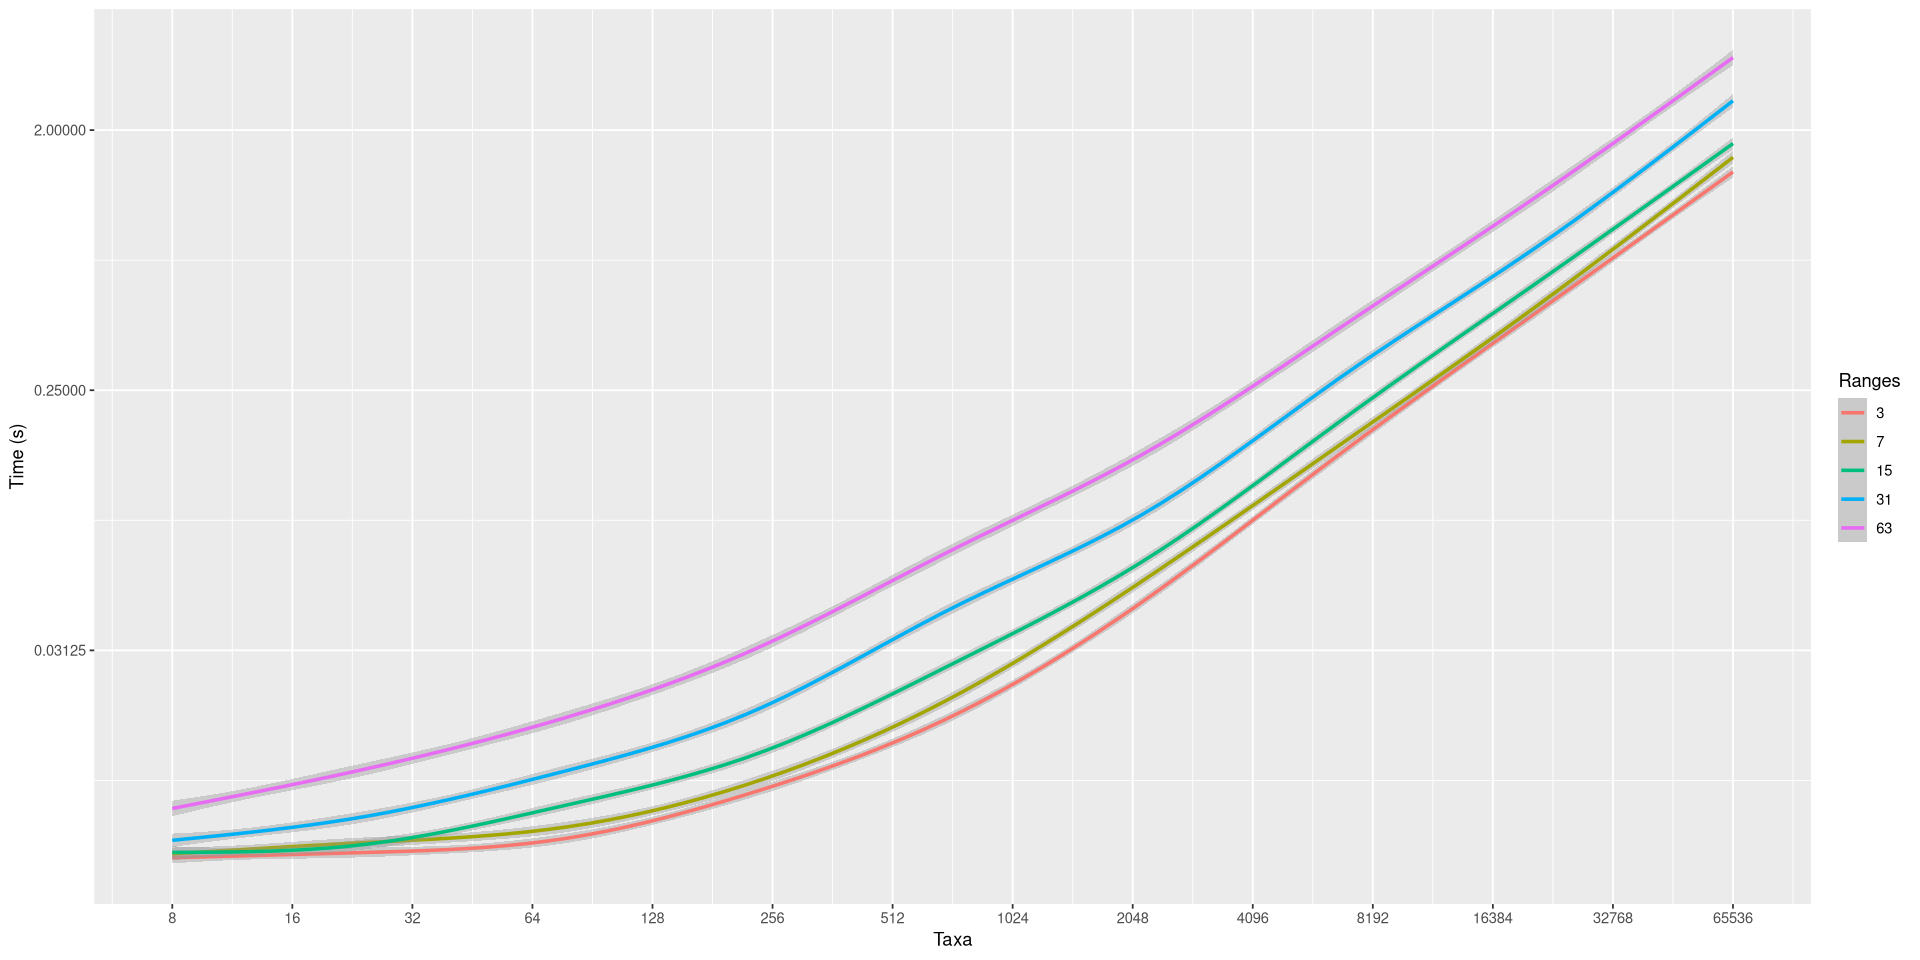
\includegraphics[width=0.95\textwidth]{figs/bigrig-runtime-taxa-loglog-plot.png}
  \end{center}
  \caption{Runtime plot}\label{fig:runtime-taxa}
\end{figure}

\begin{figure}
  \begin{center}
    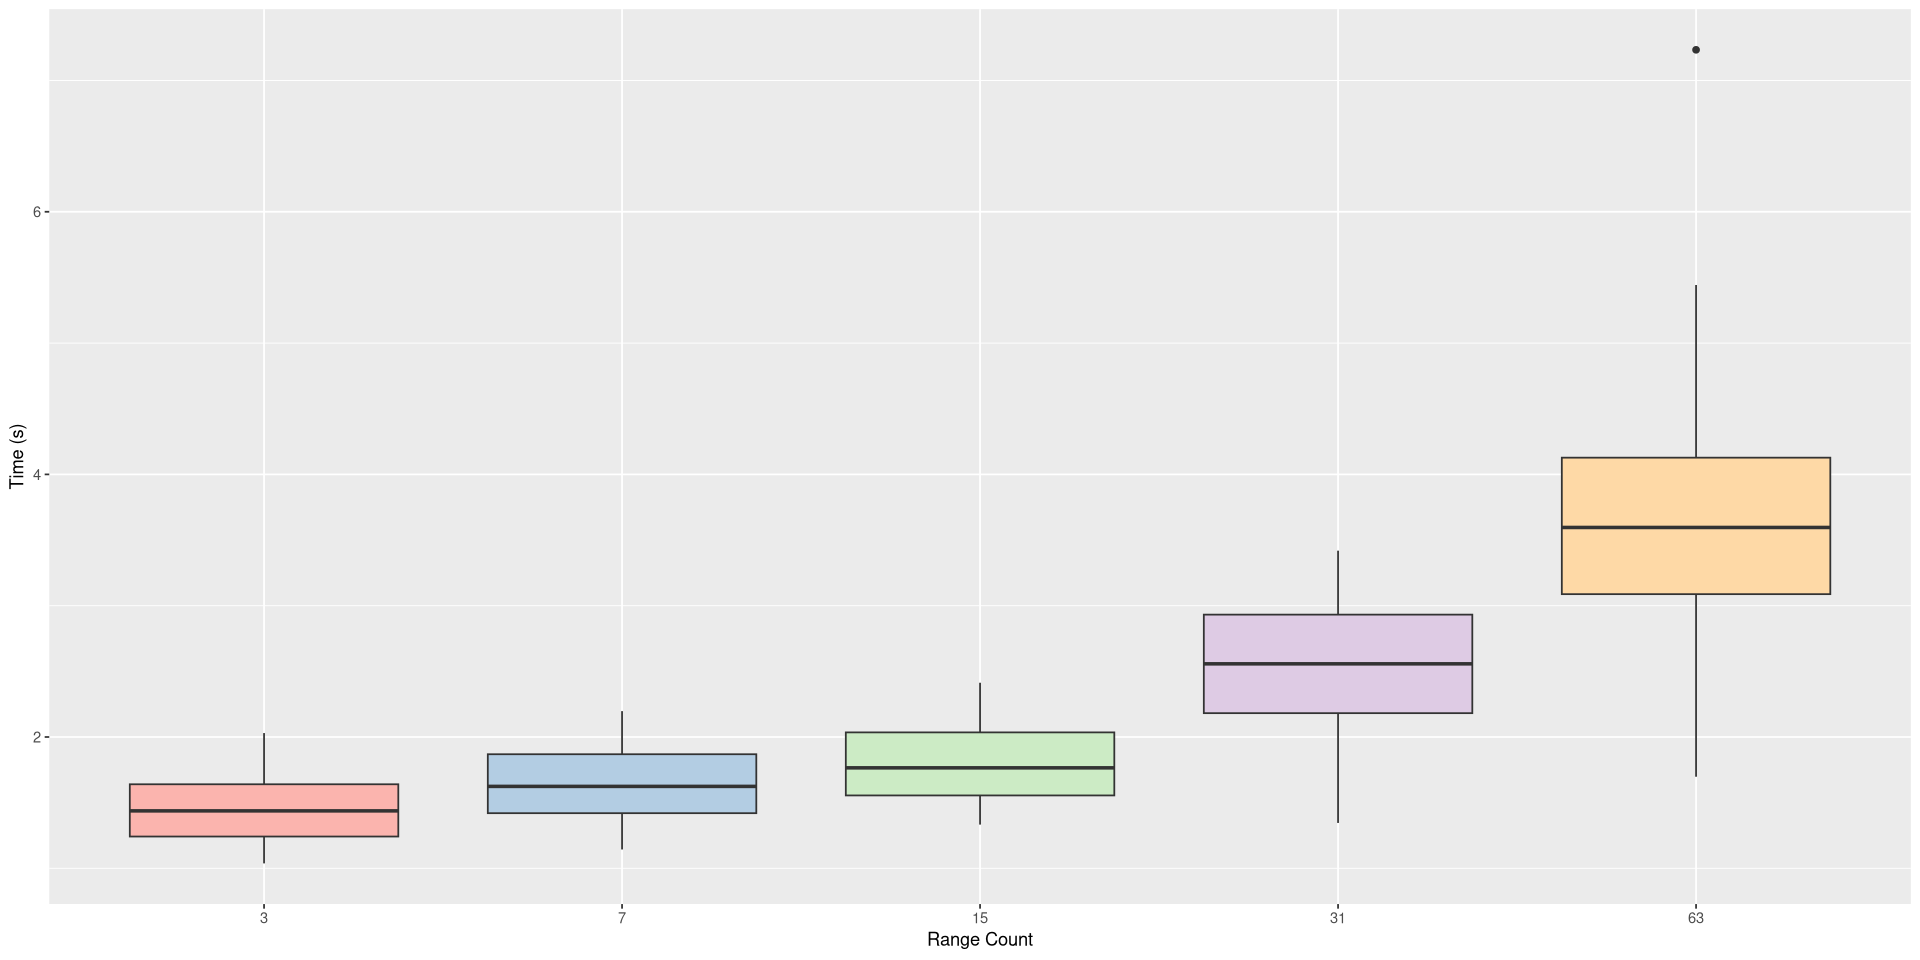
\includegraphics[width=0.95\textwidth]{figs/bigrig-runtime-range-time-boxplot.png}
  \end{center}
  \caption{Runtime plot}\label{fig:runtime-regions}
\end{figure}


\section{Conclusion}

\section{Acknowledgements}

Many thanks to Alexander I. Jordan for his assistance on deriving and
implementing the statistical tests used to verify the results of \bigrig{}.

\bibliography{references}

\end{document}
